\newpage
\section{Teoria}
\subsection{Rede $L$}
A rede L é a mais simples das redes e é largamente utilizada por isso. A rede L pode ser Passa-Baixas ou Passa-Altar, porém como neste trabalho o intuito da rede L é bloquear componentes DC, trabalharemos com a rede L Passa-Altas.

\begin{figure}[H]
    \centering
    \caption{Rede L passa-altas.}
    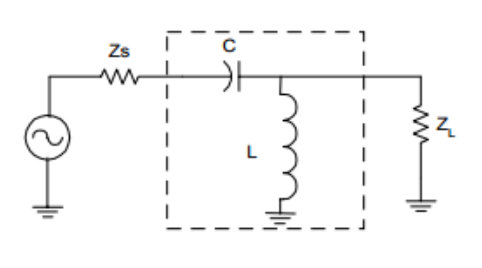
\includegraphics[scale=0.3]{Imagens/fig1.png}
    \label{f_fig1}
\end{figure}

Para o projeto de uma rede L, precisamos determinar seu valores de capacitância e indutância.

\begin{figure}[H]
    \centering
    \caption{Parâmetros da rede L.}
    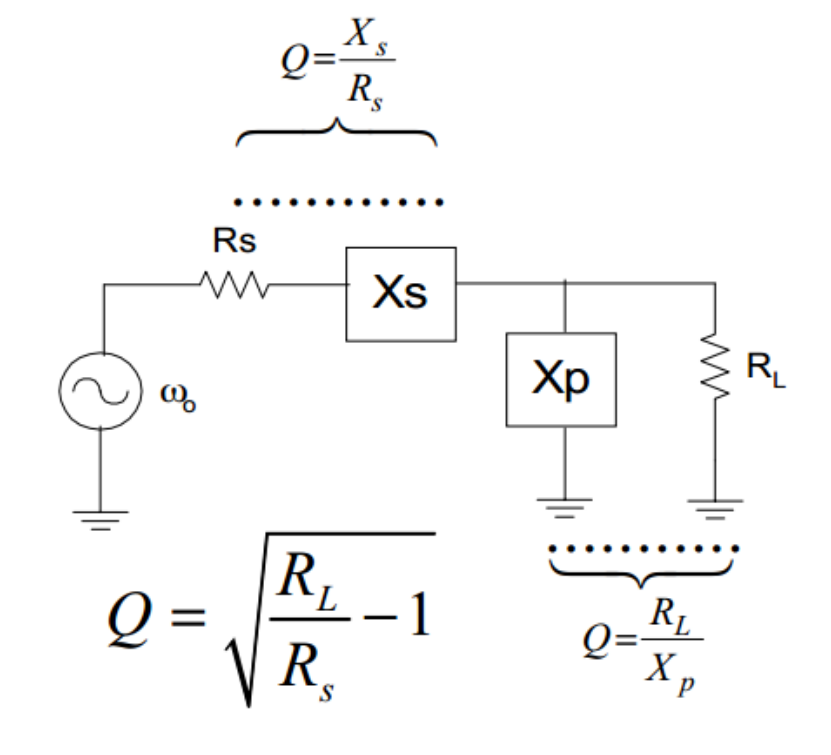
\includegraphics[scale=0.3]{Imagens/fig2.png}
    \label{f_fig2}
\end{figure}

Fator de qualidade em redes L está definido (fixo) pela relação entre $R_L$ e $R_S$ . Não há liberdade de escolha para o índice de qualidade o que é um dos grandes problemas no projeto de redes de banda estreita. Para resolver este problema, surgem as redes de três elementos que permitem obter adaptação de Z de banda estreita com alto Q.

\subsection{Rede $L_{wideband}$}

Uma vez que em uma rede L, definido $R_S$ e $R_L$, fica determinado o índice de qualidade
carregado da rede. Para adaptação de Z em circuitos de Banda Larga, usa-se duas (ou mais)
Redes L em cascata (ou série). Para esse tipo de rede adaptadora, a resistência virtual está
sempre entre os valores das resistências de fonte e carga. O índice de qualidade desse tipo de
rede é menor que os de uma rede L simples, rede T ou rede $\pi$ . O valor de Q é dado por:

\begin{equation}
Q = \sqrt{\frac{R_v}{R_{min}} -1 }
\end{equation}

onde a máxima banda de passagem ( ou mínimo Q) é obtida quando:

\begin{equation}
R_v = \sqrt{R_SR_L}
\end{equation}

Conforme a necessidade de BW seja maior, mais redes L devem ser cascateadas.
As etapas de projeto para redes WBand de n seções L são as mesmas que as anteriores:
basta solucionar a equação para um específico Q carregado baixo de projeto, obtendo RV e
seguir os passos já discutidos para uma rede L simples.


\begin{figure}[H]
    \centering
    \caption{Parâmetros da rede $L_{wideband}$.}
    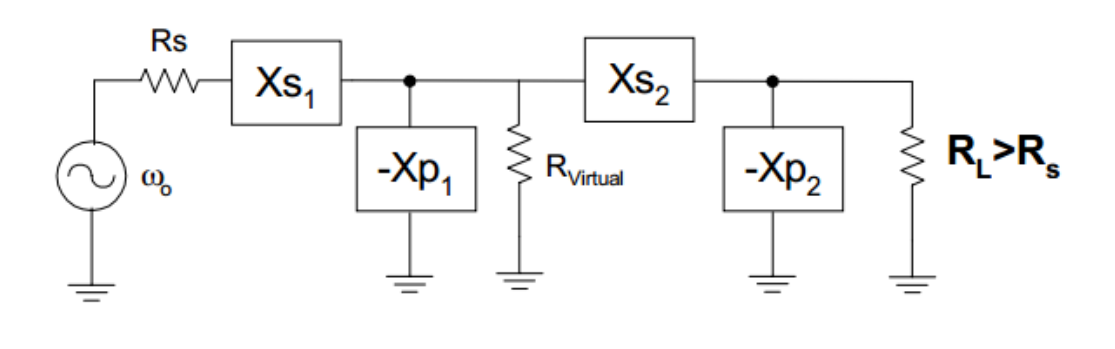
\includegraphics[scale=0.3]{Imagens/fig3.png}
    \label{f_fig3}
\end{figure}

\section{Rede T}

O projeto da rede T segue as mesmas etapas do projeto de uma rede $\pi$. Neste tipo de rede,
também deve-se adaptar a impedância da fonte à da carga via $R_{Virtual}$ . A resistência virtual
na rede T é: $R_V \ge  maxR_S ; R_L$ .

\begin{figure}[H]
    \centering
    \caption{Parâmetros da rede $T$.}
    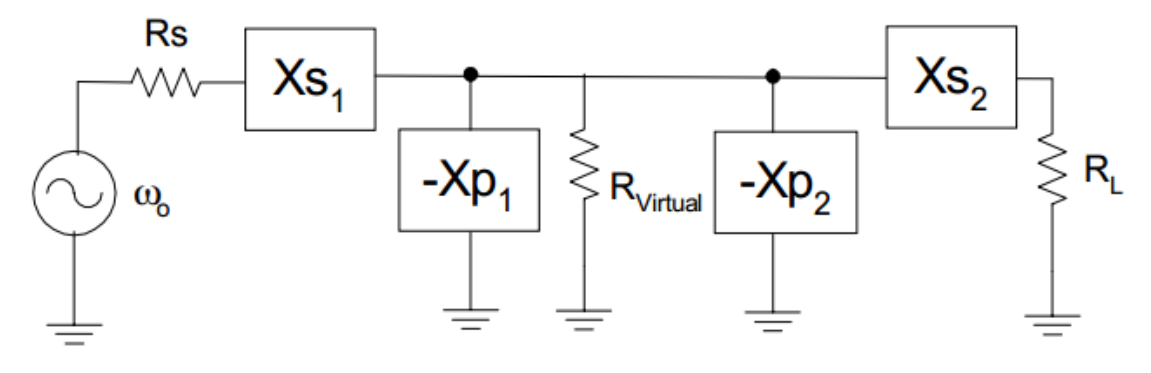
\includegraphics[scale=0.3]{Imagens/fig4.png}
    \label{f_fig4}
\end{figure}


Este tipo de rede é utilizada para adaptar duas impedâncias de baixo valor associado à
necessidade de acoplamento em banda estreita (alto Q).
Q carregado da rede T é determinado pela seção L de maior Q (isto ocorre na terminação
da seção L que tiver o menor resistor série de terminação), isto é $R_{Small}$ = $minR_S$ ; $R_L$.

\begin{equation}
Q = \sqrt{\frac{R_v}{R_{small}} -1 }
\end{equation}